\section{Results}\label{sec:results}
This section demonstrates that \textbf{FEMBA} consistently achieves \gls{soa} or near-\gls{soa} performance on diverse EEG benchmarks (TUAB, TUAR, and TUSL), while using significantly fewer FLOPs and less memory compared to recent \gls{soa} self-supervised Transformer-based methods. We provide quantitative accuracy metrics and efficiency analyses, which underscores FEMBA’s suitability for large-scale clinical or wearable EEG systems. For specific training details we fine-tune all layers (encoder + classifier) end-to-end using the Adam optimizer (initial learning rate of $1 \times 10^{-4}$) with cosine decay scheduling. Early stopping is employed based on validation loss to mitigate overfitting.

\begin{table}[h!]
    \centering
    \caption{Performance Comparison on TUAB}
    \label{tab:results_tuab}
    \resizebox{\columnwidth}{!} {
    \setlength{\tabcolsep}{6pt} 
    \begin{tabular}{@{}lcccc@{}}
        \toprule
        \textbf{Model} & \textbf{Model Size} & \textbf{Bal. Acc. (\%)} & \textbf{AUPR} & \textbf{AUROC} \\ 
        \midrule
        \textbf{Supervised Models} \\
        SPaRCNet & 0.8M & 78.96 $\pm$ 0.18 & 0.8414 $\pm$ 0.0018 & 0.8676 $\pm$ 0.0012 \\
        ContraWR & 1.6M & 77.46 $\pm$ 0.41 & 0.8421 $\pm$ 0.0140 & 0.8456 $\pm$ 0.0074 \\
        CNN-Transformer & 3.2M & 77.77 $\pm$ 0.22 & 0.8433 $\pm$ 0.0039 & 0.8461 $\pm$ 0.0013 \\
        FFCL & 2.4M & 78.48 $\pm$ 0.38 & 0.8448 $\pm$ 0.0065 & 0.8569 $\pm$ 0.0051 \\
        ST-Transformer & 3.2M & 79.66 $\pm$ 0.23 & 0.8521 $\pm$ 0.0026 & 0.8707 $\pm$ 0.0019 \\
        \midrule
        \textbf{Self-superv. Models} \\
        BENDR & 0.39M & 76.96 $\pm$ 3.98 &  & 0.8397 $\pm$ 0.0344 \\
        BrainBERT & 43.2M & - & 0.8460 $\pm$ 0.0030 & 0.8530 $\pm$ 0.0020 \\
        EEGFormer-Small & 1.9M & - & 0.8620 $\pm$ 0.0050 & 0.8620 $\pm$ 0.0070 \\
        EEGFormer-Base & 2.3M & - & 0.8670 $\pm$ 0.0020 & 0.8670 $\pm$ 0.0030 \\
        EEGFormer-Large & 3.2M & - & 0.8720 $\pm$ 0.0010 & 0.8760 $\pm$ 0.0030 \\
        BIOT & 3.2M & 79.59 $\pm$ 0.57 & 0.8692 $\pm$ 0.0023 & 0.8815 $\pm$ 0.0043 \\
        EEG2Rep & - & 80.52 $\pm$ 2.22 &  & 0.8843 $\pm$ 0.0309 \\
        LaBraM-Base & 5.8M & 81.40 $\pm$ 0.19 & 0.8965 $\pm$ 0.0016 & 0.9022 $\pm$ 0.0009 \\
        LaBraM-Large & 46M & 82.26 $\pm$ 0.15 & 0.9130 $\pm$ 0.0005 & 0.9127 $\pm$ 0.0005 \\
        LaBraM-Huge & 369M & 82.58 $\pm$ 0.11 & 0.9204 $\pm$ 0.0011 & 0.9162 $\pm$ 0.0016 \\
        \midrule
        \textbf{FEMBA-Base} & 47.7M  &81.05 $\pm$ 0.14 &0.8894 $\pm$0.0050  & 0.8829 $\pm$ 0.0021  \\
        \textbf{FEMBA-Large} & 77.8M &  81.47 $\pm$ 0.11 & 0.8992 $\pm$ 0.0007  & 0.8856 $\pm$ 0.0004 \\
        \textbf{FEMBA-Huge} & 386M  & 81.82 $\pm$ 0.16 & 0.9005 $\pm$ 0.0017 & 0.8921 $\pm$ 0.0042  \\
        \bottomrule
   \end{tabular}}
   
\end{table}
\begin{table}[b]
    \centering
    \caption{Model Comparison of FLOPs, Parameters, and Peak Memory Usage}
    \label{tab:model_comparison}
    \setlength{\tabcolsep}{6pt} 
    \renewcommand{\arraystretch}{1.2} 
    \small 
    \begin{tabular}{@{}lccc@{}}
    \toprule
    \textbf{Model} & \textbf{FLOPs} & \textbf{Parameters} & \textbf{Memory (MB)} \\ 
    \midrule
    EEGFormer-Small     & 21.06B & 1.9M     & 44.63 \\ 
    EEGFormer-Base      & 26.20B & 2.3M     & 71.32 \\ 
    EEGFormer-Large     & 36.46B & 3.2M     & 108.02 \\ 
    LaBraM-Base         & 4.42B  & 5.8M     & 757.38 \\ 
    LaBraM-Large        & 27.79B & 46M      & 1371.92 \\ 
    LaBraM-Huge         & 202.17B & 369M    & 2758.42 \\ 
    \textbf{FEMBA-Tiny} & 1.31B  & 7.8M     & 53.36 \\ 
    \textbf{FEMBA-Base} & 7.52B  & 47.7M    & 240.50 \\ 
    \textbf{FEMBA-Large} & 12.48B & 77.8M   & 548.71 \\ 
    \textbf{FEMBA-Huge} & 58.74B & 386M     & 1886.17 \\ 
    \bottomrule
    \end{tabular}
\end{table}
\begin{table*}[t]
    \centering
    \caption{Detailed Results on TUAR Across Four Classification Protocols}
    \label{tab:results_tuar}
    \small 
    \begin{tabular}{@{}lccccccc@{}}
    \toprule
    \textbf{Model} & \textbf{Model Size} & \multicolumn{2}{c}{\textbf{BC}} & \multicolumn{2}{c}{\textbf{MC}} & \multicolumn{2}{c}{\textbf{MMC}} \\
    \cmidrule(lr){3-4} \cmidrule(lr){5-6} \cmidrule(lr){7-8}
     &  & \textbf{AUROC} & \textbf{AUPR} & \textbf{AUROC} & \textbf{AUPR} & \textbf{AUROC} & \textbf{AUPR} \\
    \midrule
    \textbf{FEMBA-Tiny}  & 7.8M  
     & 0.937 $\pm$ 0.008 & 0.912 $\pm$ 0.010  
     & 0.887 $\pm$ 0.029 & 0.645 $\pm$ 0.024  
     & 0.893 $\pm$ 0.005 & 0.504 $\pm$ 0.013 
    \\
    \textbf{FEMBA-Base}  & 47.7M 
     & 0.949 $\pm$ 0.002 & 0.932 $\pm$ 0.001 
     & 0.909 $\pm$ 0.004 & 0.634 $\pm$ 0.016 
     & 0.888 $\pm$ 0.004 & 0.518 $\pm$ 0.002 
    \\
    \textbf{FEMBA-Large} & 77.8M  
     & 0.944 $\pm$ 0.003 & 0.913 $\pm$ 0.016 
     & 0.899 $\pm$ 0.006 & 0.608 $\pm$ 0.011 
     & 0.878 $\pm$ 0.020 & 0.516 $\pm$ 0.008 
    \\
    \bottomrule
    \end{tabular}
\end{table*}

\begin{table}[h!]
\centering
\caption{Performance Comparison across TUAR, TUSL}
\label{tab:results_tusl_neonate}
\resizebox{\columnwidth}{!} {
\setlength{\tabcolsep}{2pt} 
\begin{tabular}{@{}lccccccc@{}}
\toprule
\textbf{Model} & \textbf{Method Size} & \multicolumn{2}{c}{\textbf{TUAR}} & \multicolumn{2}{c}{\textbf{TUSL}} \\
\cmidrule(lr){3-4} \cmidrule(lr){5-6}
 &  & \textbf{AUROC} & \textbf{AUPR} & \textbf{AUROC} & \textbf{AUPR} \\
\midrule
EEGNet       & -  & 0.752 $\pm$ 0.006 & 0.433 $\pm$ 0.025 & 0.635 $\pm$ 0.015 & 0.351 $\pm$ 0.006  \\
TCN          & - & 0.687 $\pm$ 0.011 & 0.408 $\pm$ 0.009 & 0.545 $\pm$ 0.009 & 0.344 $\pm$ 0.001  \\
EEG-GNN      & - & 0.837 $\pm$ 0.022 & 0.488 $\pm$ 0.015 & 0.721 $\pm$ 0.009 & 0.381 $\pm$ 0.004  \\
GraphS4mer   & -  & 0.833 $\pm$ 0.006 & 0.461 $\pm$ 0.024 & 0.632 $\pm$ 0.017 & 0.359 $\pm$ 0.001  \\
BrainBERT    & 43.2M  & 0.753 $\pm$ 0.012 & 0.350 $\pm$ 0.014 & 0.588 $\pm$ 0.013 & 0.352 $\pm$ 0.003  \\
EEGFormer-Small  & 1.9M  & 0.847 $\pm$ 0.013 & 0.488 $\pm$ 0.012 & 0.683 $\pm$ 0.018 & 0.397 $\pm$ 0.011  \\
EEGFormer-Base  & 2.3M & 0.847 $\pm$ 0.014 & 0.483 $\pm$ 0.026 & 0.713 $\pm$ 0.010 & \textbf{0.393 $\pm$ 0.003}  \\
EEGFormer-Large  & 3.2M & 0.852 $\pm$ 0.004 & 0.483 $\pm$ 0.014 & 0.679 $\pm$ 0.013 & 0.389 $\pm$ 0.003  \\
\midrule
\textbf{FEMBA-Tiny}  & 7.8M  & \textbf{0.918 $\pm$ 0.003} & 0.518 $\pm$ 0.002 & 0.708 $\pm$ 0.005 & 0.277 $\pm$ 0.007 \\
\textbf{FEMBA-Base}  & 47.7M & 0.900 $\pm$ 0.010 & \textbf{0.559 $\pm$ 0.002}& \textbf{0.731 $\pm$ 0.012} & 0.289 $\pm$ 0.009\\
\textbf{FEMBA-Large} & 77.8M  & 0.915 $\pm$ 0.003 & 0.521 $\pm$ 0.001 &0.714 $\pm$ 0.007 & 0.282 $\pm$ 0.010 \\

\bottomrule
\end{tabular}
}
\end{table}
\subsection{Pre-training results}
Our FEMBA model variants are initially pretrained to reconstruct both masked and unmasked sections of the signal, as detailed in Section~\ref{subsec:pretraining}. All variants demonstrated strong reconstruction capabilities for both masked and unmasked portions of the signal. This is illustrated in Fig~\ref{fig:reconstruct}, where the FEMBA-Base model successfully reconstructs a masked signal. The training and validation loss during pretraining were closely aligned for all variants, with example loss values for FEMBA base of $0.122$ (Train) and $0.217$ (Validation).
\begin{figure}
    \centering
    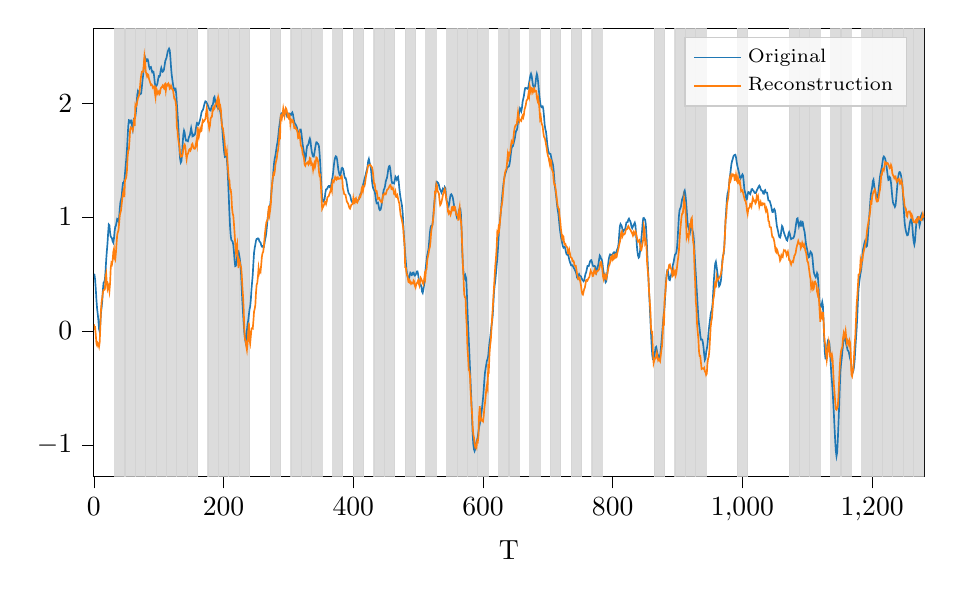
\begin{tikzpicture}

\definecolor{darkgray176}{RGB}{176,176,176}
\definecolor{darkorange25512714}{RGB}{255,127,14}
\definecolor{lightgray}{RGB}{211,211,211}
\definecolor{lightgray204}{RGB}{204,204,204}
\definecolor{steelblue31119180}{RGB}{31,119,180}

\begin{axis}[
legend cell align={left},
height=0.6\columnwidth,
width=\columnwidth,
legend style={fill opacity=0.8, draw opacity=1, text opacity=1, draw=lightgray204, font=\scriptsize},
tick align=outside,
tick pos=left,
x grid style={darkgray176},
xlabel={T},
xmin=0, xmax=1280,
xtick style={color=black},
y grid style={darkgray176},
ymin=-1.27726567983627, ymax=2.65695322751999,
ytick style={color=black}
]

\path [draw=lightgray, fill=lightgray, opacity=0.8]
(axis cs:32,-2)
--(axis cs:32,3)
--(axis cs:48,3)
--(axis cs:48,-2)
--cycle;
\path [draw=lightgray, fill=lightgray, opacity=0.8]
(axis cs:48,-2)
--(axis cs:48,3)
--(axis cs:64,3)
--(axis cs:64,-2)
--cycle;
\path [draw=lightgray, fill=lightgray, opacity=0.8]
(axis cs:64,-2)
--(axis cs:64,3)
--(axis cs:80,3)
--(axis cs:80,-2)
--cycle;
\path [draw=lightgray, fill=lightgray, opacity=0.8]
(axis cs:80,-2)
--(axis cs:80,3)
--(axis cs:96,3)
--(axis cs:96,-2)
--cycle;
\path [draw=lightgray, fill=lightgray, opacity=0.8]
(axis cs:96,-2)
--(axis cs:96,3)
--(axis cs:112,3)
--(axis cs:112,-2)
--cycle;
\path [draw=lightgray, fill=lightgray, opacity=0.8]
(axis cs:112,-2)
--(axis cs:112,3)
--(axis cs:128,3)
--(axis cs:128,-2)
--cycle;
\path [draw=lightgray, fill=lightgray, opacity=0.8]
(axis cs:128,-2)
--(axis cs:128,3)
--(axis cs:144,3)
--(axis cs:144,-2)
--cycle;
\path [draw=lightgray, fill=lightgray, opacity=0.8]
(axis cs:144,-2)
--(axis cs:144,3)
--(axis cs:160,3)
--(axis cs:160,-2)
--cycle;
\path [draw=lightgray, fill=lightgray, opacity=0.8]
(axis cs:176,-2)
--(axis cs:176,3)
--(axis cs:192,3)
--(axis cs:192,-2)
--cycle;
\path [draw=lightgray, fill=lightgray, opacity=0.8]
(axis cs:192,-2)
--(axis cs:192,3)
--(axis cs:208,3)
--(axis cs:208,-2)
--cycle;
\path [draw=lightgray, fill=lightgray, opacity=0.8]
(axis cs:208,-2)
--(axis cs:208,3)
--(axis cs:224,3)
--(axis cs:224,-2)
--cycle;
\path [draw=lightgray, fill=lightgray, opacity=0.8]
(axis cs:224,-2)
--(axis cs:224,3)
--(axis cs:240,3)
--(axis cs:240,-2)
--cycle;
\path [draw=lightgray, fill=lightgray, opacity=0.8]
(axis cs:272,-2)
--(axis cs:272,3)
--(axis cs:288,3)
--(axis cs:288,-2)
--cycle;
\path [draw=lightgray, fill=lightgray, opacity=0.8]
(axis cs:304,-2)
--(axis cs:304,3)
--(axis cs:320,3)
--(axis cs:320,-2)
--cycle;
\path [draw=lightgray, fill=lightgray, opacity=0.8]
(axis cs:320,-2)
--(axis cs:320,3)
--(axis cs:336,3)
--(axis cs:336,-2)
--cycle;
\path [draw=lightgray, fill=lightgray, opacity=0.8]
(axis cs:336,-2)
--(axis cs:336,3)
--(axis cs:352,3)
--(axis cs:352,-2)
--cycle;
\path [draw=lightgray, fill=lightgray, opacity=0.8]
(axis cs:368,-2)
--(axis cs:368,3)
--(axis cs:384,3)
--(axis cs:384,-2)
--cycle;
\path [draw=lightgray, fill=lightgray, opacity=0.8]
(axis cs:400,-2)
--(axis cs:400,3)
--(axis cs:416,3)
--(axis cs:416,-2)
--cycle;
\path [draw=lightgray, fill=lightgray, opacity=0.8]
(axis cs:432,-2)
--(axis cs:432,3)
--(axis cs:448,3)
--(axis cs:448,-2)
--cycle;
\path [draw=lightgray, fill=lightgray, opacity=0.8]
(axis cs:448,-2)
--(axis cs:448,3)
--(axis cs:464,3)
--(axis cs:464,-2)
--cycle;
\path [draw=lightgray, fill=lightgray, opacity=0.8]
(axis cs:480,-2)
--(axis cs:480,3)
--(axis cs:496,3)
--(axis cs:496,-2)
--cycle;
\path [draw=lightgray, fill=lightgray, opacity=0.8]
(axis cs:512,-2)
--(axis cs:512,3)
--(axis cs:528,3)
--(axis cs:528,-2)
--cycle;
\path [draw=lightgray, fill=lightgray, opacity=0.8]
(axis cs:544,-2)
--(axis cs:544,3)
--(axis cs:560,3)
--(axis cs:560,-2)
--cycle;
\path [draw=lightgray, fill=lightgray, opacity=0.8]
(axis cs:560,-2)
--(axis cs:560,3)
--(axis cs:576,3)
--(axis cs:576,-2)
--cycle;
\path [draw=lightgray, fill=lightgray, opacity=0.8]
(axis cs:576,-2)
--(axis cs:576,3)
--(axis cs:592,3)
--(axis cs:592,-2)
--cycle;
\path [draw=lightgray, fill=lightgray, opacity=0.8]
(axis cs:592,-2)
--(axis cs:592,3)
--(axis cs:608,3)
--(axis cs:608,-2)
--cycle;
\path [draw=lightgray, fill=lightgray, opacity=0.8]
(axis cs:624,-2)
--(axis cs:624,3)
--(axis cs:640,3)
--(axis cs:640,-2)
--cycle;
\path [draw=lightgray, fill=lightgray, opacity=0.8]
(axis cs:640,-2)
--(axis cs:640,3)
--(axis cs:656,3)
--(axis cs:656,-2)
--cycle;
\path [draw=lightgray, fill=lightgray, opacity=0.8]
(axis cs:672,-2)
--(axis cs:672,3)
--(axis cs:688,3)
--(axis cs:688,-2)
--cycle;
\path [draw=lightgray, fill=lightgray, opacity=0.8]
(axis cs:704,-2)
--(axis cs:704,3)
--(axis cs:720,3)
--(axis cs:720,-2)
--cycle;
\path [draw=lightgray, fill=lightgray, opacity=0.8]
(axis cs:736,-2)
--(axis cs:736,3)
--(axis cs:752,3)
--(axis cs:752,-2)
--cycle;
\path [draw=lightgray, fill=lightgray, opacity=0.8]
(axis cs:768,-2)
--(axis cs:768,3)
--(axis cs:784,3)
--(axis cs:784,-2)
--cycle;
\path [draw=lightgray, fill=lightgray, opacity=0.8]
(axis cs:864,-2)
--(axis cs:864,3)
--(axis cs:880,3)
--(axis cs:880,-2)
--cycle;
\path [draw=lightgray, fill=lightgray, opacity=0.8]
(axis cs:896,-2)
--(axis cs:896,3)
--(axis cs:912,3)
--(axis cs:912,-2)
--cycle;
\path [draw=lightgray, fill=lightgray, opacity=0.8]
(axis cs:912,-2)
--(axis cs:912,3)
--(axis cs:928,3)
--(axis cs:928,-2)
--cycle;
\path [draw=lightgray, fill=lightgray, opacity=0.8]
(axis cs:928,-2)
--(axis cs:928,3)
--(axis cs:944,3)
--(axis cs:944,-2)
--cycle;
\path [draw=lightgray, fill=lightgray, opacity=0.8]
(axis cs:992,-2)
--(axis cs:992,3)
--(axis cs:1008,3)
--(axis cs:1008,-2)
--cycle;
\path [draw=lightgray, fill=lightgray, opacity=0.8]
(axis cs:1072,-2)
--(axis cs:1072,3)
--(axis cs:1088,3)
--(axis cs:1088,-2)
--cycle;
\path [draw=lightgray, fill=lightgray, opacity=0.8]
(axis cs:1088,-2)
--(axis cs:1088,3)
--(axis cs:1104,3)
--(axis cs:1104,-2)
--cycle;
\path [draw=lightgray, fill=lightgray, opacity=0.8]
(axis cs:1104,-2)
--(axis cs:1104,3)
--(axis cs:1120,3)
--(axis cs:1120,-2)
--cycle;
\path [draw=lightgray, fill=lightgray, opacity=0.8]
(axis cs:1136,-2)
--(axis cs:1136,3)
--(axis cs:1152,3)
--(axis cs:1152,-2)
--cycle;
\path [draw=lightgray, fill=lightgray, opacity=0.8]
(axis cs:1152,-2)
--(axis cs:1152,3)
--(axis cs:1168,3)
--(axis cs:1168,-2)
--cycle;
\path [draw=lightgray, fill=lightgray, opacity=0.8]
(axis cs:1184,-2)
--(axis cs:1184,3)
--(axis cs:1200,3)
--(axis cs:1200,-2)
--cycle;
\path [draw=lightgray, fill=lightgray, opacity=0.8]
(axis cs:1200,-2)
--(axis cs:1200,3)
--(axis cs:1216,3)
--(axis cs:1216,-2)
--cycle;
\path [draw=lightgray, fill=lightgray, opacity=0.8]
(axis cs:1216,-2)
--(axis cs:1216,3)
--(axis cs:1232,3)
--(axis cs:1232,-2)
--cycle;
\path [draw=lightgray, fill=lightgray, opacity=0.8]
(axis cs:1232,-2)
--(axis cs:1232,3)
--(axis cs:1248,3)
--(axis cs:1248,-2)
--cycle;
\path [draw=lightgray, fill=lightgray, opacity=0.8]
(axis cs:1248,-2)
--(axis cs:1248,3)
--(axis cs:1264,3)
--(axis cs:1264,-2)
--cycle;
\path [draw=lightgray, fill=lightgray, opacity=0.8]
(axis cs:1264,-2)
--(axis cs:1264,3)
--(axis cs:1280,3)
--(axis cs:1280,-2)
--cycle;
\addplot [semithick, steelblue31119180]
table {%
0 0.5
1 0.492517083883286
2 0.449121087789536
3 0.366894543170929
4 0.272265642881393
5 0.197656258940697
6 0.149804696440697
7 0.0929687544703484
8 0.016015624627471
9 -0.00625000009313226
10 0.0699218735098839
11 0.161328122019768
12 0.206640630960464
13 0.267187505960464
14 0.364453136920929
15 0.424072265625
16 0.43017578125
17 0.450292974710464
18 0.522229015827179
19 0.619238317012787
20 0.698437511920929
21 0.765625
22 0.856640636920929
23 0.934374988079071
24 0.927343785762787
25 0.865429699420929
26 0.828320324420929
27 0.822070300579071
28 0.811328113079071
29 0.787109375
30 0.775195300579071
31 0.810351550579071
32 0.8759765625
33 0.9140625
34 0.924218773841858
35 0.952343761920929
36 0.984375
37 0.980078160762787
38 0.96484375
39 0.998046875
40 1.07539069652557
41 1.1328125
42 1.15234375
43 1.18710935115814
44 1.25468754768372
45 1.30000007152557
46 1.30312502384186
47 1.3203125
48 1.38046872615814
49 1.44765627384186
50 1.5078125
51 1.58671879768372
52 1.69296872615814
53 1.79453122615814
54 1.85000002384186
55 1.84765625
56 1.83359372615814
57 1.84765625
58 1.84843754768372
59 1.80000007152557
60 1.76953125
61 1.81171882152557
62 1.86406254768372
63 1.87265622615814
64 1.88203132152557
65 1.92890632152557
66 2.00234389305115
67 2.07343745231628
68 2.10625004768372
69 2.09531259536743
70 2.08203125
71 2.08281254768372
72 2.07890629768372
73 2.08750009536743
74 2.13906264305115
75 2.19843745231628
76 2.2421875
77 2.30937504768372
78 2.38125014305115
79 2.3984375
80 2.375
81 2.37031245231628
82 2.38437509536743
83 2.38437509536743
84 2.36093759536743
85 2.32343745231628
86 2.3046875
87 2.31562495231628
88 2.31718754768372
89 2.29062509536743
90 2.27187514305115
91 2.27812504768372
92 2.2734375
93 2.23281264305115
94 2.17656254768372
95 2.14687514305115
96 2.1484375
97 2.15625
98 2.17031264305115
99 2.20624995231628
100 2.23593759536743
101 2.23281264305115
102 2.2421875
103 2.28593754768372
104 2.30937504768372
105 2.29062509536743
106 2.27500009536743
107 2.27812504768372
108 2.29062509536743
109 2.32656264305115
110 2.3671875
111 2.3828125
112 2.39687514305115
113 2.42656254768372
114 2.453125
115 2.46718764305115
116 2.47812509536743
117 2.46406245231628
118 2.40156245231628
119 2.31562495231628
120 2.25
121 2.20624995231628
122 2.16718745231628
123 2.13125014305115
124 2.1171875
125 2.12812495231628
126 2.12812495231628
127 2.08046889305115
128 1.99296879768372
129 1.90625
130 1.82109379768372
131 1.70859372615814
132 1.58984375
133 1.51093757152557
134 1.47812497615814
135 1.48984372615814
136 1.55546879768372
137 1.64999997615814
138 1.72578132152557
139 1.75859379768372
140 1.7421875
141 1.69687497615814
142 1.671875
143 1.67343747615814
144 1.66718757152557
145 1.66484379768372
146 1.68906247615814
147 1.70781254768372
148 1.71640622615814
149 1.75234377384186
150 1.78125
151 1.75
152 1.70781254768372
153 1.71015632152557
154 1.72265625
155 1.71875
156 1.72890627384186
157 1.76250004768372
158 1.80078125
159 1.82578122615814
160 1.82187497615814
161 1.80937504768372
162 1.81796872615814
163 1.83984375
164 1.85859382152557
165 1.88671875
166 1.91796875
167 1.93124997615814
168 1.9375
169 1.95625007152557
170 1.98046875
171 2.00234389305115
172 2.015625
173 2.01328134536743
174 2.00156259536743
175 1.99140632152557
176 1.97578132152557
177 1.95937502384186
178 1.94921875
179 1.9375
180 1.93437504768372
181 1.95625007152557
182 1.9765625
183 1.97890627384186
184 2.00078129768372
185 2.04453134536743
186 2.05390620231628
187 2.02265620231628
188 1.99453127384186
189 1.98046875
190 1.96875
191 1.95625007152557
192 1.95000004768372
193 1.94921875
194 1.94453132152557
195 1.921875
196 1.88750004768372
197 1.84218752384186
198 1.7734375
199 1.69453132152557
200 1.62656247615814
201 1.56718754768372
202 1.52812504768372
203 1.53125
204 1.54531252384186
205 1.515625
206 1.43437504768372
207 1.31875002384186
208 1.18085944652557
209 1.04062497615814
210 0.919921875
211 0.835546910762787
212 0.798046886920929
213 0.7919921875
214 0.784375011920929
215 0.754296898841858
216 0.694042980670929
217 0.617968738079071
218 0.568798840045929
219 0.572021484375
220 0.609570324420929
221 0.657421886920929
222 0.695898473262787
223 0.699902355670929
224 0.670117199420929
225 0.6337890625
226 0.586865246295929
227 0.496740728616714
228 0.371386736631393
229 0.256249994039536
230 0.1611328125
231 0.0691406279802322
232 -0.0105468751862645
233 -0.0671875029802322
234 -0.0984375029802322
235 -0.0730468779802322
236 0.00507812527939677
237 0.0640624985098839
238 0.0925781279802322
239 0.140625
240 0.188281252980232
241 0.21484375
242 0.272265642881393
243 0.361230462789536
244 0.428515642881393
245 0.49615478515625
246 0.598095715045929
247 0.686914086341858
248 0.728515625
249 0.758593738079071
250 0.793164074420929
251 0.808007836341858
252 0.8076171875
253 0.813281238079071
254 0.809765636920929
255 0.790625035762787
256 0.781445324420929
257 0.775781273841858
258 0.754296898841858
259 0.741601586341858
260 0.744726598262787
261 0.7373046875
262 0.736328125
263 0.7666015625
264 0.8017578125
265 0.827539086341858
266 0.869140625
267 0.929296910762787
268 0.987890660762787
269 1.03398442268372
270 1.06406247615814
271 1.08203125
272 1.111328125
273 1.16835939884186
274 1.23671877384186
275 1.294921875
276 1.34843754768372
277 1.41562497615814
278 1.48046875
279 1.51796877384186
280 1.54218757152557
281 1.58125007152557
282 1.62265622615814
283 1.65078127384186
284 1.69140625
285 1.75
286 1.79843747615814
287 1.83749997615814
288 1.87968754768372
289 1.90781247615814
290 1.91250002384186
291 1.90781247615814
292 1.89765632152557
293 1.89140629768372
294 1.90781247615814
295 1.93359375
296 1.9296875
297 1.89999997615814
298 1.8828125
299 1.890625
300 1.90312504768372
301 1.90937507152557
302 1.90703129768372
303 1.89687502384186
304 1.89531254768372
305 1.90937507152557
306 1.91796875
307 1.90078127384186
308 1.86484372615814
309 1.83437502384186
310 1.8203125
311 1.81328129768372
312 1.80312502384186
313 1.78828132152557
314 1.76171875
315 1.73593747615814
316 1.73281252384186
317 1.74921882152557
318 1.76718747615814
319 1.76796877384186
320 1.73671877384186
321 1.68359375
322 1.63515627384186
323 1.60000002384186
324 1.5703125
325 1.53359377384186
326 1.50859379768372
327 1.53515625
328 1.59531247615814
329 1.62734377384186
330 1.63046872615814
331 1.64453125
332 1.67343747615814
333 1.68906247615814
334 1.66718757152557
335 1.61406254768372
336 1.57187497615814
337 1.55000007152557
338 1.53125
339 1.52968752384186
340 1.55937504768372
341 1.59687507152557
342 1.63046872615814
343 1.65625
344 1.65546882152557
345 1.64296877384186
346 1.640625
347 1.62265622615814
348 1.56093752384186
349 1.46953129768372
350 1.36562502384186
351 1.25703132152557
352 1.17460942268372
353 1.14140629768372
354 1.134765625
355 1.13593757152557
356 1.16523444652557
357 1.21601569652557
358 1.24257814884186
359 1.24374997615814
360 1.25156247615814
361 1.26523435115814
362 1.27187502384186
363 1.27187502384186
364 1.26015627384186
365 1.25742185115814
366 1.28789067268372
367 1.32421875
368 1.35000002384186
369 1.39218747615814
370 1.45078122615814
371 1.49453127384186
372 1.51953125
373 1.53281247615814
374 1.52968752384186
375 1.50703132152557
376 1.46015632152557
377 1.41328132152557
378 1.38750004768372
379 1.36796879768372
380 1.36171877384186
381 1.39296877384186
382 1.42812502384186
383 1.43203127384186
384 1.42500007152557
385 1.40703129768372
386 1.36796879768372
387 1.34453129768372
388 1.34375
389 1.32890629768372
390 1.29453122615814
391 1.25820314884186
392 1.22734379768372
393 1.20703125
394 1.20000004768372
395 1.19140625
396 1.16835939884186
397 1.14296877384186
398 1.13320314884186
399 1.13632810115814
400 1.13945317268372
401 1.138671875
402 1.13593757152557
403 1.13632810115814
404 1.13671875
405 1.13125002384186
406 1.13164067268372
407 1.14414060115814
408 1.15273439884186
409 1.16015625
410 1.18281257152557
411 1.203125
412 1.20859372615814
413 1.22617185115814
414 1.26015627384186
415 1.28398442268372
416 1.30234372615814
417 1.328125
418 1.34843754768372
419 1.36874997615814
420 1.39609372615814
421 1.41562497615814
422 1.44453132152557
423 1.49374997615814
424 1.51015627384186
425 1.48046875
426 1.45781254768372
427 1.43515622615814
428 1.37578129768372
429 1.30859375
430 1.267578125
431 1.24648439884186
432 1.23710942268372
433 1.22539067268372
434 1.19296872615814
435 1.1484375
436 1.12070310115814
437 1.12343752384186
438 1.12617194652557
439 1.10078132152557
440 1.0703125
441 1.060546875
442 1.06523442268372
443 1.08515632152557
444 1.12070310115814
445 1.16289067268372
446 1.20820319652557
447 1.23984372615814
448 1.25
449 1.27265632152557
450 1.31015622615814
451 1.32968747615814
452 1.34531247615814
453 1.38203132152557
454 1.42109382152557
455 1.44453132152557
456 1.44843757152557
457 1.42265629768372
458 1.37109375
459 1.31875002384186
460 1.29726564884186
461 1.30156254768372
462 1.29804694652557
463 1.294921875
464 1.32343757152557
465 1.35390627384186
466 1.34453129768372
467 1.32968747615814
468 1.34531247615814
469 1.35312497615814
470 1.3125
471 1.25117194652557
472 1.201171875
473 1.16367185115814
474 1.13359379768372
475 1.10195314884186
476 1.04726564884186
477 0.955859363079071
478 0.846093773841858
479 0.752148449420929
480 0.679394543170929
481 0.606640636920929
482 0.538793981075287
483 0.497235119342804
484 0.471704095602036
485 0.453833013772964
486 0.462060540914536
487 0.491973876953125
488 0.511627197265625
489 0.506292760372162
490 0.491259783506393
491 0.494085699319839
492 0.512719750404358
493 0.513293445110321
494 0.494412243366241
495 0.486010760068893
496 0.492266863584518
497 0.505529820919037
498 0.522534191608429
499 0.523388683795929
500 0.495062261819839
501 0.451318353414536
502 0.412988275289536
503 0.400537103414536
504 0.406201183795929
505 0.387597650289536
506 0.345898449420929
507 0.334179699420929
508 0.361425787210464
509 0.399511724710464
510 0.450268566608429
511 0.514196813106537
512 0.571240246295929
513 0.622168004512787
514 0.666308581829071
515 0.6904296875
516 0.719531238079071
517 0.783007800579071
518 0.855078160762787
519 0.90234375
520 0.921875
521 0.923437535762787
522 0.933203160762787
523 0.982812523841858
524 1.06093752384186
525 1.12968754768372
526 1.18476569652557
527 1.24296879768372
528 1.29257810115814
529 1.30937504768372
530 1.3046875
531 1.29843747615814
532 1.28085935115814
533 1.25429689884186
534 1.240234375
535 1.22773444652557
536 1.21367192268372
537 1.2265625
538 1.24609375
539 1.236328125
540 1.23515629768372
541 1.26250004768372
542 1.25273442268372
543 1.19140625
544 1.14492189884186
545 1.12851560115814
546 1.10859382152557
547 1.095703125
548 1.11835944652557
549 1.16289067268372
550 1.19492185115814
551 1.20039069652557
552 1.19179689884186
553 1.17890632152557
554 1.15156257152557
555 1.111328125
556 1.08320319652557
557 1.07070314884186
558 1.04843747615814
559 1.01445317268372
560 0.992578148841858
561 0.999218761920929
562 1.02851569652557
563 1.05937504768372
564 1.07695317268372
565 1.076171875
566 1.02265632152557
567 0.880273461341858
568 0.700585961341858
569 0.575878918170929
570 0.510485827922821
571 0.465576171875
572 0.457177728414536
573 0.483056634664536
574 0.462329119443893
575 0.346386730670929
576 0.187304690480232
577 0.048828125
578 -0.0691406279802322
579 -0.198437497019768
580 -0.339062511920929
581 -0.470312505960464
582 -0.6015625
583 -0.753125011920929
584 -0.896875023841858
585 -0.990625023841858
586 -1.03750002384186
587 -1.05312502384186
588 -1.03437507152557
589 -0.995312511920929
590 -0.967187523841858
591 -0.952343761920929
592 -0.925000011920929
593 -0.882031261920929
594 -0.84375
595 -0.815625011920929
596 -0.786718785762787
597 -0.749218761920929
598 -0.701562523841858
599 -0.6484375
600 -0.592187523841858
601 -0.521093785762787
602 -0.435156255960464
603 -0.3671875
604 -0.328906267881393
605 -0.294140636920929
606 -0.260937511920929
607 -0.24609375
608 -0.219921872019768
609 -0.158593758940697
610 -0.1015625
611 -0.0632812529802322
612 -0.0105468751862645
613 0.0460937507450581
614 0.0824218764901161
615 0.138867184519768
616 0.245703130960464
617 0.347949236631393
618 0.402294933795929
619 0.444677740335464
620 0.507000744342804
621 0.572656273841858
622 0.635937511920929
623 0.718554675579071
624 0.818554699420929
625 0.905078113079071
626 0.96484375
627 1.01640629768372
628 1.07929694652557
629 1.14882814884186
630 1.2109375
631 1.26445317268372
632 1.31171882152557
633 1.34843754768372
634 1.37265622615814
635 1.390625
636 1.40937507152557
637 1.42890632152557
638 1.43984377384186
639 1.44062507152557
640 1.4453125
641 1.46796882152557
642 1.5078125
643 1.55937504768372
644 1.60390627384186
645 1.61796879768372
646 1.62109375
647 1.64140629768372
648 1.66640627384186
649 1.68906247615814
650 1.7265625
651 1.75625002384186
652 1.76171875
653 1.78359377384186
654 1.83749997615814
655 1.88906252384186
656 1.92890632152557
657 1.95546877384186
658 1.94687497615814
659 1.9296875
660 1.95781254768372
661 2.00937509536743
662 2.03671884536743
663 2.06171870231628
664 2.10468745231628
665 2.13125014305115
666 2.1328125
667 2.13125014305115
668 2.12656259536743
669 2.125
670 2.14374995231628
671 2.17656254768372
672 2.2109375
673 2.2421875
674 2.2578125
675 2.23906254768372
676 2.19687509536743
677 2.15781259536743
678 2.14374995231628
679 2.140625
680 2.14531254768372
681 2.17656254768372
682 2.22812509536743
683 2.25625014305115
684 2.23593759536743
685 2.18281245231628
686 2.12031245231628
687 2.06093764305115
688 2.01015639305115
689 1.97500002384186
690 1.96562504768372
691 1.97187507152557
692 1.97187507152557
693 1.9453125
694 1.88515627384186
695 1.81328129768372
696 1.77265632152557
697 1.75234377384186
698 1.70625007152557
699 1.64375007152557
700 1.60234379768372
701 1.57421875
702 1.5546875
703 1.55546879768372
704 1.55390632152557
705 1.52890622615814
706 1.49921882152557
707 1.48046875
708 1.45468747615814
709 1.40234375
710 1.32890629768372
711 1.26171875
712 1.21757817268372
713 1.17109382152557
714 1.11289060115814
715 1.06875002384186
716 1.03593754768372
717 0.984375
718 0.921875
719 0.872460961341858
720 0.833398461341858
721 0.80078125
722 0.773046910762787
723 0.745898425579071
724 0.732617199420929
725 0.740039050579071
726 0.740234375
727 0.717578113079071
728 0.68896484375
729 0.671093761920929
730 0.669043004512787
731 0.670703113079071
732 0.652929723262787
733 0.623925805091858
734 0.605371117591858
735 0.589404284954071
736 0.574755847454071
737 0.575976550579071
738 0.577197253704071
739 0.564062535762787
740 0.553613305091858
741 0.545556664466858
742 0.530712902545929
743 0.51904296875
744 0.500693142414093
745 0.468676775693893
746 0.461645513772964
747 0.487744152545929
748 0.499136358499527
749 0.487475603818893
750 0.482629388570786
751 0.479052752256393
752 0.463183611631393
753 0.450366228818893
754 0.444580078125
755 0.436572283506393
756 0.443017572164536
757 0.474633783102036
758 0.501623570919037
759 0.5142822265625
760 0.540551781654358
761 0.570068359375
762 0.571923851966858
763 0.569726586341858
764 0.589550793170929
765 0.610058605670929
766 0.619921863079071
767 0.621679723262787
768 0.604296863079071
769 0.579003930091858
770 0.568798840045929
771 0.568505883216858
772 0.570361316204071
773 0.565722644329071
774 0.538378894329071
775 0.51495361328125
776 0.532421886920929
777 0.565087914466858
778 0.590136706829071
779 0.628710925579071
780 0.661914050579071
781 0.653515636920929
782 0.633984386920929
783 0.628613293170929
784 0.601757824420929
785 0.54931640625
786 0.5130615234375
787 0.491101086139679
788 0.45654296875
789 0.427880853414536
790 0.435937494039536
791 0.477563470602036
792 0.535473644733429
793 0.591992199420929
794 0.632714867591858
795 0.658886730670929
796 0.672265648841858
797 0.668749988079071
798 0.6611328125
799 0.665234386920929
800 0.675683617591858
801 0.685644567012787
802 0.691308617591858
803 0.684472680091858
804 0.673730492591858
805 0.680566430091858
806 0.702734410762787
807 0.71875
808 0.729101598262787
809 0.766992211341858
810 0.846289098262787
811 0.918749988079071
812 0.938281238079071
813 0.929296910762787
814 0.91796875
815 0.892382800579071
816 0.8720703125
817 0.881250023841858
818 0.890039086341858
819 0.891015648841858
820 0.918749988079071
821 0.952343761920929
822 0.954296886920929
823 0.955468773841858
824 0.977734386920929
825 0.985937535762787
826 0.97265625
827 0.962890625
828 0.944921910762787
829 0.913671910762787
830 0.901953160762787
831 0.915234386920929
832 0.927343785762787
833 0.938671886920929
834 0.950390636920929
835 0.926953136920929
836 0.851757824420929
837 0.761914074420929
838 0.698144555091858
839 0.66259765625
840 0.643457055091858
841 0.650000035762787
842 0.694628894329071
843 0.755273461341858
844 0.805273473262787
845 0.8623046875
846 0.9375
847 0.989062488079071
848 0.991796910762787
849 0.982031285762787
850 0.975390613079071
851 0.935546875
852 0.841992199420929
853 0.719140648841858
854 0.590624988079071
855 0.4647216796875
856 0.345800787210464
857 0.229882821440697
858 0.1083984375
859 -0.0164062511175871
860 -0.130859375
861 -0.212890625
862 -0.248437508940697
863 -0.249609380960464
864 -0.230859383940697
865 -0.189062505960464
866 -0.145703122019768
867 -0.139453127980232
868 -0.169140622019768
869 -0.199609383940697
870 -0.215625002980232
871 -0.227343752980232
872 -0.236328125
873 -0.219531252980232
874 -0.167187497019768
875 -0.103515625
876 -0.0382812507450581
877 0.0375000014901161
878 0.1064453125
879 0.157812505960464
880 0.224023446440697
881 0.322656244039536
882 0.424462884664536
883 0.496995538473129
884 0.5328369140625
885 0.5311279296875
886 0.492864996194839
887 0.449902355670929
888 0.445996105670929
889 0.471215814352036
890 0.491314709186554
891 0.5166015625
892 0.555810570716858
893 0.584570348262787
894 0.607324242591858
895 0.642187535762787
896 0.669238269329071
897 0.676367223262787
898 0.688183605670929
899 0.7255859375
900 0.798437535762787
901 0.903906285762787
902 1.00468754768372
903 1.05937504768372
904 1.07421875
905 1.087890625
906 1.12265622615814
907 1.15703129768372
908 1.17031252384186
909 1.18710935115814
910 1.21992194652557
911 1.23203122615814
912 1.20000004768372
913 1.14179694652557
914 1.06406247615814
915 0.974609375
916 0.919531285762787
917 0.904296875
918 0.880078136920929
919 0.863476574420929
920 0.907031238079071
921 0.953515648841858
922 0.927343785762787
923 0.880859375
924 0.8603515625
925 0.808007836341858
926 0.703710973262787
927 0.598876953125
928 0.505059838294983
929 0.40869140625
930 0.313769549131393
931 0.213671877980232
932 0.119531251490116
933 0.0609375014901161
934 0.017578125
935 -0.0386718772351742
936 -0.0750000029802322
937 -0.0734375044703484
938 -0.0757812485098839
939 -0.101953126490116
940 -0.144921883940697
941 -0.205859377980232
942 -0.252734392881393
943 -0.238671883940697
944 -0.189453125
945 -0.157812505960464
946 -0.124609373509884
947 -0.060546875
948 0.00625000009313226
949 0.0539062507450581
950 0.100390627980232
951 0.147656247019768
952 0.173632815480232
953 0.191015630960464
954 0.246875002980232
955 0.348730474710464
956 0.451123058795929
957 0.531762719154358
958 0.593408226966858
959 0.608593761920929
960 0.571142613887787
961 0.527075231075287
962 0.485217303037643
963 0.428320318460464
964 0.392382830381393
965 0.400634765625
966 0.419482439756393
967 0.451464861631393
968 0.52978515625
969 0.619921863079071
970 0.659863293170929
971 0.674218773841858
972 0.741015613079071
973 0.860742211341858
974 0.971875011920929
975 1.06523442268372
976 1.15468752384186
977 1.20546877384186
978 1.22226560115814
979 1.26328122615814
980 1.32343757152557
981 1.36953127384186
982 1.41640627384186
983 1.46562504768372
984 1.49140632152557
985 1.50859379768372
986 1.53125
987 1.54140627384186
988 1.54531252384186
989 1.546875
990 1.52578127384186
991 1.48671877384186
992 1.453125
993 1.42734372615814
994 1.40468752384186
995 1.37968754768372
996 1.35000002384186
997 1.33828127384186
998 1.35000002384186
999 1.36406254768372
1000 1.37421882152557
1001 1.36171877384186
1002 1.30390632152557
1003 1.24101567268372
1004 1.21640622615814
1005 1.19140625
1006 1.15390622615814
1007 1.15859377384186
1008 1.19843757152557
1009 1.21992194652557
1010 1.21757817268372
1011 1.20664060115814
1012 1.20078122615814
1013 1.21992194652557
1014 1.24453127384186
1015 1.24531257152557
1016 1.23593747615814
1017 1.23007810115814
1018 1.22031247615814
1019 1.21132814884186
1020 1.21015632152557
1021 1.216796875
1022 1.23085939884186
1023 1.24453127384186
1024 1.25507819652557
1025 1.26835942268372
1026 1.27578127384186
1027 1.26601564884186
1028 1.24687504768372
1029 1.23281252384186
1030 1.23125004768372
1031 1.2265625
1032 1.20664060115814
1033 1.20429694652557
1034 1.22968757152557
1035 1.23554694652557
1036 1.21562504768372
1037 1.21367192268372
1038 1.21406257152557
1039 1.18007814884186
1040 1.14609372615814
1041 1.14414060115814
1042 1.14140629768372
1043 1.12187504768372
1044 1.1015625
1045 1.07421875
1046 1.044921875
1047 1.04414069652557
1048 1.06328129768372
1049 1.0703125
1050 1.05937504768372
1051 1.02734375
1052 0.971484363079071
1053 0.922656238079071
1054 0.897851586341858
1055 0.872265636920929
1056 0.841210961341858
1057 0.823632836341858
1058 0.820117175579071
1059 0.838476598262787
1060 0.885156273841858
1061 0.921093761920929
1062 0.911718785762787
1063 0.883203148841858
1064 0.86328125
1065 0.845703125
1066 0.830078125
1067 0.816796898841858
1068 0.799023449420929
1069 0.794140636920929
1070 0.819531261920929
1071 0.854101598262787
1072 0.8681640625
1073 0.853320300579071
1074 0.822851598262787
1075 0.806250035762787
1076 0.810546875
1077 0.814257800579071
1078 0.813671886920929
1079 0.821679711341858
1080 0.839648425579071
1081 0.870898425579071
1082 0.912890613079071
1083 0.951953113079071
1084 0.983593761920929
1085 0.988671898841858
1086 0.949609398841858
1087 0.919921875
1088 0.941796898841858
1089 0.952734410762787
1090 0.922656238079071
1091 0.922656238079071
1092 0.958984375
1093 0.955468773841858
1094 0.914843738079071
1095 0.888867199420929
1096 0.861718773841858
1097 0.810546875
1098 0.761914074420929
1099 0.732812523841858
1100 0.707812488079071
1101 0.674609363079071
1102 0.645898461341858
1103 0.64892578125
1104 0.678906261920929
1105 0.695410192012787
1106 0.689160168170929
1107 0.677343785762787
1108 0.641015648841858
1109 0.571972668170929
1110 0.516699254512787
1111 0.496652215719223
1112 0.482873529195786
1113 0.470996111631393
1114 0.483850091695786
1115 0.509167492389679
1116 0.496990978717804
1117 0.420166015625
1118 0.316601574420929
1119 0.245898440480232
1120 0.217968747019768
1121 0.2119140625
1122 0.228320315480232
1123 0.2548828125
1124 0.224414065480232
1125 0.0953124985098839
1126 -0.0687500014901161
1127 -0.185156255960464
1128 -0.241796880960464
1129 -0.242968752980232
1130 -0.182812497019768
1131 -0.108984373509884
1132 -0.0804687514901161
1133 -0.0847656279802322
1134 -0.106640629470348
1135 -0.17578125
1136 -0.282812505960464
1137 -0.373437494039536
1138 -0.442968755960464
1139 -0.525781273841858
1140 -0.626562535762787
1141 -0.733593761920929
1142 -0.8515625
1143 -0.967187523841858
1144 -1.05546879768372
1145 -1.09843754768372
1146 -1.06718754768372
1147 -0.95703125
1148 -0.817187488079071
1149 -0.671093761920929
1150 -0.500781238079071
1151 -0.35546875
1152 -0.287109375
1153 -0.242968752980232
1154 -0.180859372019768
1155 -0.126171872019768
1156 -0.07421875
1157 -0.02734375
1158 -0.0359374992549419
1159 -0.0855468735098839
1160 -0.118359379470348
1161 -0.140625
1162 -0.166406258940697
1163 -0.174218758940697
1164 -0.184375002980232
1165 -0.217578127980232
1166 -0.242968752980232
1167 -0.261328130960464
1168 -0.307031244039536
1169 -0.35546875
1170 -0.365624994039536
1171 -0.348437517881393
1172 -0.31640625
1173 -0.252734392881393
1174 -0.159374997019768
1175 -0.068359375
1176 0.0148437498137355
1177 0.124609373509884
1178 0.262500017881393
1179 0.368847668170929
1180 0.422705084085464
1181 0.46630859375
1182 0.506878674030304
1183 0.535376012325287
1184 0.589404284954071
1185 0.669335961341858
1186 0.718554675579071
1187 0.740234375
1188 0.772070348262787
1189 0.789453148841858
1190 0.767773449420929
1191 0.741601586341858
1192 0.747265636920929
1193 0.795312523841858
1194 0.879296898841858
1195 0.967187523841858
1196 1.04531252384186
1197 1.12929689884186
1198 1.19921875
1199 1.22929692268372
1200 1.26171875
1201 1.31484377384186
1202 1.32734382152557
1203 1.28242194652557
1204 1.2421875
1205 1.22226560115814
1206 1.19453132152557
1207 1.16875004768372
1208 1.16875004768372
1209 1.19570314884186
1210 1.24492192268372
1211 1.30390632152557
1212 1.35312497615814
1213 1.38671875
1214 1.4140625
1215 1.44375002384186
1216 1.48515629768372
1217 1.52109372615814
1218 1.53125
1219 1.52421879768372
1220 1.51171875
1221 1.48750007152557
1222 1.44921875
1223 1.40625
1224 1.359375
1225 1.32500004768372
1226 1.32890629768372
1227 1.35078132152557
1228 1.34375
1229 1.30078125
1230 1.24101567268372
1231 1.17617189884186
1232 1.12890625
1233 1.11328125
1234 1.10390627384186
1235 1.08945310115814
1236 1.10234379768372
1237 1.15703129768372
1238 1.22773444652557
1239 1.29296875
1240 1.34687507152557
1241 1.38046872615814
1242 1.39453125
1243 1.39296877384186
1244 1.37578129768372
1245 1.34609377384186
1246 1.30546879768372
1247 1.24179685115814
1248 1.1484375
1249 1.04257810115814
1250 0.955859363079071
1251 0.905859410762787
1252 0.878320336341858
1253 0.8544921875
1254 0.839257836341858
1255 0.841601550579071
1256 0.8642578125
1257 0.90625
1258 0.947656273841858
1259 0.970703125
1260 0.98046875
1261 0.966796875
1262 0.910937488079071
1263 0.8369140625
1264 0.7802734375
1265 0.758398473262787
1266 0.791015625
1267 0.869531273841858
1268 0.94140625
1269 0.978515625
1270 0.999218761920929
1271 1.00078129768372
1272 0.964062511920929
1273 0.925390660762787
1274 0.948437511920929
1275 1.0078125
1276 1.02187502384186
1277 0.992968738079071
1278 0.982031285762787
1279 1.00898444652557
};
\addlegendentry{Original}
\addplot [semithick, darkorange25512714]
table {%
0 0.0588483512401581
1 0.0231761336326599
2 0.028899610042572
3 -0.0336881279945374
4 -0.110973179340363
5 -0.126554846763611
6 -0.104747623205185
7 -0.113265514373779
8 -0.136740684509277
9 -0.0988295674324036
10 0.037085235118866
11 0.183905765414238
12 0.259652733802795
13 0.290320098400116
14 0.340510874986649
15 0.361066281795502
16 0.360537141561508
17 0.364173620939255
18 0.474528908729553
19 0.502542674541473
20 0.417700469493866
21 0.374718368053436
22 0.405448436737061
23 0.385372221469879
24 0.348254323005676
25 0.419089913368225
26 0.549782514572144
27 0.595917344093323
28 0.58532726764679
29 0.618478298187256
30 0.694074869155884
31 0.719208955764771
32 0.637398362159729
33 0.625084280967712
34 0.685483813285828
35 0.770482897758484
36 0.84257173538208
37 0.867789387702942
38 0.884118795394897
39 0.945396900177002
40 1.01552700996399
41 1.03818011283875
42 1.06165063381195
43 1.11670029163361
44 1.16938233375549
45 1.21013760566711
46 1.23491525650024
47 1.1750602722168
48 1.32168769836426
49 1.33289432525635
50 1.34883975982666
51 1.4062180519104
52 1.52305853366852
53 1.58276617527008
54 1.59232521057129
55 1.67163991928101
56 1.76939678192139
57 1.78523302078247
58 1.77667284011841
59 1.77535653114319
60 1.76001560688019
61 1.79434287548065
62 1.86347305774689
63 1.80061566829681
64 1.98353850841522
65 1.97072660923004
66 1.98393929004669
67 2.01426887512207
68 2.04317951202393
69 2.054518699646
70 2.0755512714386
71 2.1313955783844
72 2.1965229511261
73 2.24602603912354
74 2.27467966079712
75 2.27444458007812
76 2.27476811408997
77 2.33689188957214
78 2.41317415237427
79 2.37266778945923
80 2.27669978141785
81 2.25751185417175
82 2.23604202270508
83 2.25307416915894
84 2.24730610847473
85 2.21408748626709
86 2.19546818733215
87 2.1788866519928
88 2.15945100784302
89 2.1633665561676
90 2.15676951408386
91 2.13598132133484
92 2.14350295066833
93 2.14603090286255
94 2.09391593933105
95 2.05585598945618
96 2.13009238243103
97 2.11787033081055
98 2.08289170265198
99 2.09271860122681
100 2.10125231742859
101 2.07831525802612
102 2.08692097663879
103 2.12632441520691
104 2.13698935508728
105 2.14148664474487
106 2.15271162986755
107 2.13934588432312
108 2.1308708190918
109 2.16345977783203
110 2.16884851455688
111 2.11060881614685
112 2.14683270454407
113 2.16340136528015
114 2.15759038925171
115 2.17131948471069
116 2.16004848480225
117 2.12502694129944
118 2.13050293922424
119 2.15114760398865
120 2.13288259506226
121 2.11947870254517
122 2.11620306968689
123 2.07803320884705
124 2.03875327110291
125 2.03601217269897
126 2.0135669708252
127 1.96513438224792
128 1.78318655490875
129 1.76238787174225
130 1.68929648399353
131 1.65102648735046
132 1.61724901199341
133 1.55898380279541
134 1.52960848808289
135 1.53295755386353
136 1.53303050994873
137 1.55487310886383
138 1.59790730476379
139 1.62676239013672
140 1.6367723941803
141 1.61856842041016
142 1.55437064170837
143 1.5086327791214
144 1.5448009967804
145 1.55582165718079
146 1.57130575180054
147 1.5919361114502
148 1.59794509410858
149 1.58483982086182
150 1.5973881483078
151 1.63577497005463
152 1.64259564876556
153 1.6192215681076
154 1.60529851913452
155 1.59888303279877
156 1.60045373439789
157 1.63206648826599
158 1.66304802894592
159 1.63428676128387
160 1.79004597663879
161 1.7511533498764
162 1.70799624919891
163 1.73912572860718
164 1.7757523059845
165 1.75242388248444
166 1.75719380378723
167 1.81984400749207
168 1.84698891639709
169 1.83551895618439
170 1.84295547008514
171 1.85236215591431
172 1.8601747751236
173 1.9095094203949
174 1.95299315452576
175 1.91367793083191
176 1.83736801147461
177 1.81648397445679
178 1.77684056758881
179 1.8014829158783
180 1.86419939994812
181 1.87657248973846
182 1.87977766990662
183 1.92987835407257
184 1.9582222700119
185 1.94417500495911
186 1.95311987400055
187 1.98257958889008
188 1.9899001121521
189 2.00533056259155
190 2.024174451828
191 1.98235440254211
192 2.04889631271362
193 2.02593326568604
194 1.95762884616852
195 1.97066080570221
196 1.93643724918365
197 1.83060503005981
198 1.78790402412415
199 1.78027260303497
200 1.7338855266571
201 1.69383347034454
202 1.63203561306
203 1.54549741744995
204 1.54750764369965
205 1.57812476158142
206 1.48585510253906
207 1.41387152671814
208 1.33641147613525
209 1.32320618629456
210 1.24439465999603
211 1.241002202034
212 1.1955498456955
213 1.08146870136261
214 1.03275978565216
215 1.01171815395355
216 0.940024495124817
217 0.85771107673645
218 0.763677597045898
219 0.692404270172119
220 0.732490301132202
221 0.761098265647888
222 0.629259169101715
223 0.552414298057556
224 0.623164534568787
225 0.607352256774902
226 0.57660585641861
227 0.561540961265564
228 0.495607376098633
229 0.387899696826935
230 0.308315008878708
231 0.19162854552269
232 0.0196305811405182
233 -0.0752946436405182
234 -0.0863812267780304
235 -0.133064419031143
236 -0.166316658258438
237 -0.107449620962143
238 -0.0130065381526947
239 0.0732352286577225
240 -0.0810426473617554
241 -0.109069555997849
242 -0.0473825335502625
243 0.0189541280269623
244 0.0262711644172668
245 0.0220927894115448
246 0.0896842181682587
247 0.170846730470657
248 0.193701073527336
249 0.230023786425591
250 0.337091028690338
251 0.406648725271225
252 0.421652227640152
253 0.47988885641098
254 0.551545202732086
255 0.509580969810486
256 0.530337870121002
257 0.519778728485107
258 0.578420579433441
259 0.648024678230286
260 0.682023286819458
261 0.692832887172699
262 0.734874904155731
263 0.804007232189178
264 0.864264965057373
265 0.91275429725647
266 0.955299377441406
267 0.964707016944885
268 0.982088685035706
269 1.05122458934784
270 1.099081158638
271 1.02930343151093
272 1.0676931142807
273 1.12443029880524
274 1.2358078956604
275 1.29632806777954
276 1.3506406545639
277 1.38358879089355
278 1.37479615211487
279 1.40034234523773
280 1.46365368366241
281 1.49022722244263
282 1.51263988018036
283 1.56071245670319
284 1.59036874771118
285 1.63580560684204
286 1.71837043762207
287 1.68248426914215
288 1.8887996673584
289 1.89515280723572
290 1.87070691585541
291 1.90753793716431
292 1.95146012306213
293 1.91766405105591
294 1.8853931427002
295 1.92160511016846
296 1.95537924766541
297 1.94552505016327
298 1.91511702537537
299 1.87912333011627
300 1.87027788162231
301 1.90006411075592
302 1.89081943035126
303 1.81564700603485
304 1.85234522819519
305 1.85577511787415
306 1.83842873573303
307 1.84450781345367
308 1.82238936424255
309 1.78086054325104
310 1.77868092060089
311 1.78582406044006
312 1.77108478546143
313 1.76517510414124
314 1.74116337299347
315 1.69198286533356
316 1.69510865211487
317 1.73058092594147
318 1.69410622119904
319 1.62887716293335
320 1.61814546585083
321 1.60067927837372
322 1.55202829837799
323 1.54056179523468
324 1.51321566104889
325 1.45930802822113
326 1.45029830932617
327 1.46882331371307
328 1.46889913082123
329 1.47750306129456
330 1.48220574855804
331 1.46096312999725
332 1.47081398963928
333 1.51800632476807
334 1.51275825500488
335 1.46364223957062
336 1.47292768955231
337 1.45997250080109
338 1.41562736034393
339 1.45398080348969
340 1.47333085536957
341 1.44201827049255
342 1.46917688846588
343 1.52297818660736
344 1.51848125457764
345 1.50311863422394
346 1.47717463970184
347 1.40101516246796
348 1.36251378059387
349 1.36772382259369
350 1.28336358070374
351 1.17667508125305
352 1.07212662696838
353 1.08439826965332
354 1.09693598747253
355 1.11050045490265
356 1.13413238525391
357 1.13050675392151
358 1.11424767971039
359 1.13571405410767
360 1.17109930515289
361 1.17834234237671
362 1.18212878704071
363 1.20009922981262
364 1.21392786502838
365 1.23400568962097
366 1.25840139389038
367 1.23292255401611
368 1.32249522209167
369 1.31858491897583
370 1.3091607093811
371 1.32874023914337
372 1.34870576858521
373 1.33369708061218
374 1.32815957069397
375 1.34909892082214
376 1.35005080699921
377 1.33450412750244
378 1.33479654788971
379 1.3380833864212
380 1.33840465545654
381 1.35356247425079
382 1.35978960990906
383 1.33104491233826
384 1.25106310844421
385 1.2309775352478
386 1.20120978355408
387 1.19837367534637
388 1.195521235466
389 1.1646044254303
390 1.13629448413849
391 1.12757134437561
392 1.1181788444519
393 1.10024070739746
394 1.08027517795563
395 1.07383596897125
396 1.0899840593338
397 1.10865044593811
398 1.11066150665283
399 1.11149573326111
400 1.16219115257263
401 1.12567591667175
402 1.12171161174774
403 1.16054058074951
404 1.16648149490356
405 1.13310241699219
406 1.1268036365509
407 1.14153838157654
408 1.15105581283569
409 1.17019760608673
410 1.18292951583862
411 1.17707669734955
412 1.2011638879776
413 1.25321054458618
414 1.26389706134796
415 1.23228657245636
416 1.26631581783295
417 1.26826655864716
418 1.29073548316956
419 1.33400869369507
420 1.36895084381104
421 1.39224636554718
422 1.42521417140961
423 1.45300936698914
424 1.45532369613647
425 1.45516812801361
426 1.45999920368195
427 1.4508171081543
428 1.4407811164856
429 1.43569421768188
430 1.4029129743576
431 1.34774398803711
432 1.29323577880859
433 1.28984677791595
434 1.24464476108551
435 1.22601354122162
436 1.22763073444366
437 1.19368422031403
438 1.16120052337646
439 1.16733741760254
440 1.16850864887238
441 1.15003252029419
442 1.1398960351944
443 1.13328313827515
444 1.12858974933624
445 1.15634751319885
446 1.19589757919312
447 1.19404792785645
448 1.20638656616211
449 1.20157885551453
450 1.19910109043121
451 1.21805024147034
452 1.23866653442383
453 1.2433168888092
454 1.24859511852264
455 1.26129508018494
456 1.273801445961
457 1.28064107894897
458 1.26883721351624
459 1.24437761306763
460 1.24240374565125
461 1.25498259067535
462 1.23796331882477
463 1.19881427288055
464 1.19679272174835
465 1.21930241584778
466 1.17606675624847
467 1.1743369102478
468 1.18879115581512
469 1.16244864463806
470 1.13739538192749
471 1.11762130260468
472 1.06548893451691
473 1.01795887947083
474 0.996771097183228
475 0.969448924064636
476 0.939472794532776
477 0.900575518608093
478 0.815921306610107
479 0.763159871101379
480 0.559436917304993
481 0.55660080909729
482 0.5107342004776
483 0.490638196468353
484 0.472041070461273
485 0.43106472492218
486 0.426525712013245
487 0.44397047162056
488 0.429038017988205
489 0.414718389511108
490 0.423457264900208
491 0.416548252105713
492 0.416071027517319
493 0.443128138780594
494 0.435468673706055
495 0.396978825330734
496 0.382056593894958
497 0.407851785421371
498 0.418479472398758
499 0.430818676948547
500 0.444085955619812
501 0.416931480169296
502 0.39864718914032
503 0.43477538228035
504 0.465446919202805
505 0.453629851341248
506 0.439837455749512
507 0.423629760742188
508 0.41037905216217
509 0.443156957626343
510 0.487335681915283
511 0.462454080581665
512 0.534475207328796
513 0.541389644145966
514 0.621128439903259
515 0.651952028274536
516 0.678651571273804
517 0.716127753257751
518 0.735465109348297
519 0.781763792037964
520 0.863935828208923
521 0.906519889831543
522 0.927095055580139
523 0.976998329162598
524 1.03370714187622
525 1.10929620265961
526 1.21739184856415
527 1.21467113494873
528 1.28975093364716
529 1.27624559402466
530 1.2294534444809
531 1.21781659126282
532 1.20542740821838
533 1.14604103565216
534 1.10464644432068
535 1.11394369602203
536 1.13302600383759
537 1.15718817710876
538 1.18917572498322
539 1.21249735355377
540 1.23256635665894
541 1.24650859832764
542 1.21684980392456
543 1.17153382301331
544 1.13331973552704
545 1.10049152374268
546 1.04930424690247
547 1.03319656848907
548 1.05041253566742
549 1.04440188407898
550 1.02255284786224
551 1.0419807434082
552 1.08647835254669
553 1.0894923210144
554 1.05771577358246
555 1.05825924873352
556 1.09051263332367
557 1.08653438091278
558 1.04319536685944
559 1.01903736591339
560 1.02160477638245
561 1.01825225353241
562 0.968239426612854
563 1.05132365226746
564 1.08548629283905
565 1.00691080093384
566 0.962078928947449
567 0.892109394073486
568 0.722524523735046
569 0.573275685310364
570 0.452426135540009
571 0.322285026311874
572 0.297354102134705
573 0.295317143201828
574 0.131089016795158
575 0.0381945073604584
576 -0.148644626140594
577 -0.229572623968124
578 -0.341072529554367
579 -0.349366337060928
580 -0.399662166833878
581 -0.545409798622131
582 -0.638921022415161
583 -0.710565328598022
584 -0.830889940261841
585 -0.907736301422119
586 -0.931702971458435
587 -0.989905118942261
588 -1.01905262470245
589 -1.00559866428375
590 -1.02021288871765
591 -0.963114261627197
592 -0.970987439155579
593 -0.918283820152283
594 -0.731083512306213
595 -0.660766124725342
596 -0.73032808303833
597 -0.785001635551453
598 -0.777799487113953
599 -0.785837411880493
600 -0.793202042579651
601 -0.750590682029724
602 -0.680631518363953
603 -0.634276032447815
604 -0.579317569732666
605 -0.513808369636536
606 -0.477571398019791
607 -0.503128051757812
608 -0.32435330748558
609 -0.340428203344345
610 -0.200104624032974
611 -0.125515818595886
612 -0.0826309621334076
613 0.0127382278442383
614 0.112762287259102
615 0.195361658930779
616 0.295549988746643
617 0.389023274183273
618 0.484640419483185
619 0.578112423419952
620 0.642332077026367
621 0.729369521141052
622 0.864978075027466
623 0.853230237960815
624 0.907443761825562
625 0.889779806137085
626 0.943997025489807
627 1.01829063892365
628 1.0754371881485
629 1.10547685623169
630 1.14703571796417
631 1.22320222854614
632 1.2985258102417
633 1.34903073310852
634 1.39065647125244
635 1.40986144542694
636 1.41783726215363
637 1.47132802009583
638 1.53520393371582
639 1.48622274398804
640 1.55740904808044
641 1.54910385608673
642 1.57237684726715
643 1.62476921081543
644 1.66221368312836
645 1.64993143081665
646 1.64793515205383
647 1.70065486431122
648 1.75709986686707
649 1.78612458705902
650 1.80488240718842
651 1.808873295784
652 1.81260287761688
653 1.86390602588654
654 1.91817533969879
655 1.8747181892395
656 1.83887040615082
657 1.85466682910919
658 1.85215699672699
659 1.84557712078094
660 1.87507843971252
661 1.88880109786987
662 1.87364649772644
663 1.89718770980835
664 1.94314634799957
665 1.96220755577087
666 1.98395013809204
667 2.02154493331909
668 2.02914428710938
669 2.03869009017944
670 2.07840800285339
671 2.05689454078674
672 2.15118527412415
673 2.12950563430786
674 2.10078024864197
675 2.13076519966125
676 2.12874317169189
677 2.09551024436951
678 2.10970997810364
679 2.12543320655823
680 2.1030158996582
681 2.10768842697144
682 2.10585737228394
683 2.04870271682739
684 2.02290463447571
685 2.04709076881409
686 2.01071739196777
687 1.94664299488068
688 1.86375141143799
689 1.88248932361603
690 1.8337117433548
691 1.8107818365097
692 1.79449284076691
693 1.74294173717499
694 1.70443618297577
695 1.69661462306976
696 1.67460596561432
697 1.64239645004272
698 1.60891401767731
699 1.56764340400696
700 1.53875720500946
701 1.5259040594101
702 1.49118518829346
703 1.46347713470459
704 1.50292432308197
705 1.49714636802673
706 1.42231464385986
707 1.40736293792725
708 1.38899648189545
709 1.31806969642639
710 1.28309631347656
711 1.28257918357849
712 1.2445672750473
713 1.1945925951004
714 1.15002107620239
715 1.09902834892273
716 1.07989799976349
717 1.07348430156708
718 1.00858116149902
719 0.967956781387329
720 0.901044249534607
721 0.857437252998352
722 0.81374454498291
723 0.835957050323486
724 0.828677415847778
725 0.773838043212891
726 0.759524464607239
727 0.763467788696289
728 0.745194315910339
729 0.740977108478546
730 0.728672921657562
731 0.68321418762207
732 0.680087208747864
733 0.70957624912262
734 0.68007755279541
735 0.649868726730347
736 0.643258094787598
737 0.639046192169189
738 0.614031612873077
739 0.617178618907928
740 0.609394431114197
741 0.576167345046997
742 0.570161283016205
743 0.571919083595276
744 0.539710998535156
745 0.501165986061096
746 0.476257920265198
747 0.453677475452423
748 0.455595314502716
749 0.463464558124542
750 0.429689258337021
751 0.402882963418961
752 0.355254590511322
753 0.32612943649292
754 0.31977653503418
755 0.343222856521606
756 0.367474615573883
757 0.380481541156769
758 0.412201166152954
759 0.446215152740479
760 0.449271649122238
761 0.442690223455429
762 0.456170797348022
763 0.465577602386475
764 0.472980558872223
765 0.502650141716003
766 0.529707431793213
767 0.516108751296997
768 0.509071946144104
769 0.482094347476959
770 0.484151661396027
771 0.522773087024689
772 0.537917017936707
773 0.50929456949234
774 0.501479029655457
775 0.521521747112274
776 0.528731167316437
777 0.527152419090271
778 0.534209489822388
779 0.541895270347595
780 0.56572687625885
781 0.601031482219696
782 0.60522449016571
783 0.580255150794983
784 0.537748694419861
785 0.47741687297821
786 0.454225480556488
787 0.488959819078445
788 0.496678471565247
789 0.459157079458237
790 0.454854488372803
791 0.484068393707275
792 0.509802103042603
793 0.541709780693054
794 0.572353720664978
795 0.581100761890411
796 0.604698479175568
797 0.646605253219604
798 0.652810573577881
799 0.63048779964447
800 0.654461622238159
801 0.629592955112457
802 0.635581374168396
803 0.668219983577728
804 0.672321915626526
805 0.644231200218201
806 0.648461699485779
807 0.681906700134277
808 0.705539107322693
809 0.728943824768066
810 0.759499192237854
811 0.780234098434448
812 0.813437044620514
813 0.863212466239929
814 0.873834371566772
815 0.831401228904724
816 0.845682740211487
817 0.850444555282593
818 0.848441481590271
819 0.858214735984802
820 0.884102463722229
821 0.893937945365906
822 0.89483916759491
823 0.910720109939575
824 0.920575976371765
825 0.907680511474609
826 0.895974516868591
827 0.890861868858337
828 0.879587650299072
829 0.866658329963684
830 0.857008695602417
831 0.840052127838135
832 0.863965749740601
833 0.848674774169922
834 0.863357186317444
835 0.874985456466675
836 0.857793927192688
837 0.827334403991699
838 0.800596117973328
839 0.783344388008118
840 0.789704561233521
841 0.795987725257874
842 0.761756062507629
843 0.714309930801392
844 0.709547877311707
845 0.737722039222717
846 0.772050857543945
847 0.803353071212769
848 0.917791604995728
849 0.891220450401306
850 0.773173809051514
851 0.789406657218933
852 0.745166480541229
853 0.596913993358612
854 0.531636774539948
855 0.472954750061035
856 0.344991952180862
857 0.269376337528229
858 0.1853988468647
859 0.0293122828006744
860 -0.0142385065555573
861 -0.0105981528759003
862 -0.18965682387352
863 -0.282246738672256
864 -0.259908348321915
865 -0.240439385175705
866 -0.241216689348221
867 -0.222390621900558
868 -0.192113608121872
869 -0.223636358976364
870 -0.256668418645859
871 -0.246286541223526
872 -0.252233058214188
873 -0.264404445886612
874 -0.216642767190933
875 -0.166491866111755
876 -0.131571710109711
877 -0.0265483558177948
878 0.0839329063892365
879 0.0468607544898987
880 0.280835181474686
881 0.32438662648201
882 0.404297858476639
883 0.473526060581207
884 0.523696839809418
885 0.534394919872284
886 0.54534637928009
887 0.580628156661987
888 0.584102034568787
889 0.554406106472015
890 0.548446536064148
891 0.527158260345459
892 0.480844616889954
893 0.486934572458267
894 0.53022837638855
895 0.505051076412201
896 0.518486857414246
897 0.487075984477997
898 0.508182466030121
899 0.553269505500793
900 0.607229292392731
901 0.648169875144958
902 0.702552199363708
903 0.794323205947876
904 0.880795359611511
905 0.939545154571533
906 0.999335646629333
907 1.03112006187439
908 1.03206646442413
909 1.08317291736603
910 1.1621071100235
911 1.12333083152771
912 1.06947505474091
913 0.961612462997437
914 0.827337384223938
915 0.852125644683838
916 0.851210832595825
917 0.817249417304993
918 0.880828976631165
919 0.929732918739319
920 0.922414422035217
921 0.980521321296692
922 0.991791725158691
923 0.859066367149353
924 0.781882524490356
925 0.750416278839111
926 0.561591684818268
927 0.43840566277504
928 0.260548770427704
929 0.205215096473694
930 0.0607544481754303
931 -0.00632199645042419
932 -0.0671767592430115
933 -0.17772251367569
934 -0.219946891069412
935 -0.21924689412117
936 -0.278404027223587
937 -0.331518977880478
938 -0.326208978891373
939 -0.329526990652084
940 -0.332778483629227
941 -0.323825508356094
942 -0.355129390954971
943 -0.355050176382065
944 -0.384962767362595
945 -0.373824626207352
946 -0.285180240869522
947 -0.242750197649002
948 -0.225365608930588
949 -0.17166656255722
950 -0.0666542649269104
951 0.0368320047855377
952 0.0854490995407104
953 0.114593639969826
954 0.198597818613052
955 0.275989383459091
956 0.304640561342239
957 0.359683781862259
958 0.434405088424683
959 0.381474703550339
960 0.474353730678558
961 0.441772878170013
962 0.450007379055023
963 0.456626385450363
964 0.466482698917389
965 0.475716829299927
966 0.485803544521332
967 0.507766008377075
968 0.546579003334045
969 0.592988848686218
970 0.648660957813263
971 0.693011581897736
972 0.734870493412018
973 0.839998364448547
974 0.982489228248596
975 0.997599720954895
976 1.10655605792999
977 1.14028322696686
978 1.16575860977173
979 1.23251700401306
980 1.33419382572174
981 1.3558257818222
982 1.32636225223541
983 1.34635138511658
984 1.37378549575806
985 1.36568069458008
986 1.37295651435852
987 1.36926937103271
988 1.32487368583679
989 1.32680630683899
990 1.36921310424805
991 1.32507526874542
992 1.31135272979736
993 1.34622156620026
994 1.30637645721436
995 1.29571461677551
996 1.31156229972839
997 1.27328753471375
998 1.22539865970612
999 1.2289731502533
1000 1.23428952693939
1001 1.21131312847137
1002 1.18601298332214
1003 1.16406309604645
1004 1.14420580863953
1005 1.13680768013
1006 1.10623097419739
1007 1.05716800689697
1008 1.02846276760101
1009 1.06932938098907
1010 1.07889568805695
1011 1.08315706253052
1012 1.1173849105835
1013 1.11567914485931
1014 1.0956062078476
1015 1.13085913658142
1016 1.16682481765747
1017 1.1505126953125
1018 1.14045631885529
1019 1.14365303516388
1020 1.12079846858978
1021 1.13023579120636
1022 1.18126821517944
1023 1.16472673416138
1024 1.18120384216309
1025 1.14083433151245
1026 1.09270250797272
1027 1.11562216281891
1028 1.13179981708527
1029 1.10452330112457
1030 1.10286939144135
1031 1.11832165718079
1032 1.11364901065826
1033 1.11997210979462
1034 1.11786198616028
1035 1.0754588842392
1036 1.05464851856232
1037 1.0765585899353
1038 1.06031489372253
1039 1.02792537212372
1040 0.964226722717285
1041 0.961544394493103
1042 0.914408564567566
1043 0.910212635993958
1044 0.90961217880249
1045 0.860579967498779
1046 0.825083494186401
1047 0.824333786964417
1048 0.812631249427795
1049 0.787007331848145
1050 0.749628305435181
1051 0.702814102172852
1052 0.692432880401611
1053 0.7176114320755
1054 0.705095529556274
1055 0.678847312927246
1056 0.665280699729919
1057 0.655818939208984
1058 0.618177652359009
1059 0.629347026348114
1060 0.663093090057373
1061 0.650775194168091
1062 0.647039771080017
1063 0.687471628189087
1064 0.709494471549988
1065 0.704301953315735
1066 0.706253409385681
1067 0.691611468791962
1068 0.666334927082062
1069 0.680925369262695
1070 0.695705890655518
1071 0.664551377296448
1072 0.622554063796997
1073 0.62224417924881
1074 0.600246965885162
1075 0.584221243858337
1076 0.603880882263184
1077 0.612237215042114
1078 0.606553256511688
1079 0.629467964172363
1080 0.660882234573364
1081 0.668531775474548
1082 0.684515953063965
1083 0.721810102462769
1084 0.746576607227325
1085 0.766961812973022
1086 0.788566768169403
1087 0.770389378070831
1088 0.764565765857697
1089 0.767608284950256
1090 0.728797852993011
1091 0.74417644739151
1092 0.770220279693604
1093 0.746353566646576
1094 0.739600419998169
1095 0.759343385696411
1096 0.738405108451843
1097 0.704368650913239
1098 0.689621329307556
1099 0.653052508831024
1100 0.612562894821167
1101 0.603903114795685
1102 0.571981310844421
1103 0.52954888343811
1104 0.48550671339035
1105 0.456433862447739
1106 0.37604159116745
1107 0.396643608808517
1108 0.416370093822479
1109 0.364000648260117
1110 0.370908439159393
1111 0.430410832166672
1112 0.43381655216217
1113 0.419702589511871
1114 0.406649798154831
1115 0.346156507730484
1116 0.319940119981766
1117 0.344369828701019
1118 0.2731973528862
1119 0.171295329928398
1120 0.0804046094417572
1121 0.158071234822273
1122 0.122855350375175
1123 0.113131180405617
1124 0.167878001928329
1125 0.104837074875832
1126 -0.0396182239055634
1127 -0.0997945070266724
1128 -0.121007800102234
1129 -0.199731677770615
1130 -0.254419595003128
1131 -0.211585730314255
1132 -0.133127927780151
1133 -0.0949311554431915
1134 -0.137565851211548
1135 -0.215253919363022
1136 -0.207410007715225
1137 -0.237123876810074
1138 -0.21102973818779
1139 -0.246137648820877
1140 -0.361377567052841
1141 -0.472775548696518
1142 -0.543730616569519
1143 -0.62300705909729
1144 -0.685075163841248
1145 -0.690826058387756
1146 -0.677505493164062
1147 -0.659262537956238
1148 -0.575515270233154
1149 -0.44224026799202
1150 -0.316416889429092
1151 -0.232285231351852
1152 -0.176226258277893
1153 -0.156034678220749
1154 -0.138438820838928
1155 -0.0646107792854309
1156 -0.0241888165473938
1157 -0.0533434748649597
1158 -0.0325586795806885
1159 0.000335276126861572
1160 -0.0556652545928955
1161 -0.105852484703064
1162 -0.0825983881950378
1163 -0.0962170660495758
1164 -0.119026035070419
1165 -0.0834437310695648
1166 -0.103661268949509
1167 -0.201705724000931
1168 -0.382050186395645
1169 -0.397042125463486
1170 -0.361611932516098
1171 -0.325798124074936
1172 -0.224011331796646
1173 -0.119050025939941
1174 -0.0410360395908356
1175 0.0896444767713547
1176 0.229151874780655
1177 0.300156354904175
1178 0.393391966819763
1179 0.493087440729141
1180 0.498115330934525
1181 0.514196276664734
1182 0.613287627696991
1183 0.578381061553955
1184 0.623386561870575
1185 0.620055615901947
1186 0.671382546424866
1187 0.698927283287048
1188 0.723162353038788
1189 0.752034187316895
1190 0.776093602180481
1191 0.818558931350708
1192 0.877246022224426
1193 0.915991306304932
1194 0.948472619056702
1195 0.985970616340637
1196 1.01222109794617
1197 1.05737483501434
1198 1.13051462173462
1199 1.12383079528809
1200 1.17719638347626
1201 1.20332515239716
1202 1.22193515300751
1203 1.22869777679443
1204 1.24166119098663
1205 1.21600985527039
1206 1.16167163848877
1207 1.13674378395081
1208 1.13633847236633
1209 1.14157795906067
1210 1.17180681228638
1211 1.21365344524384
1212 1.23919451236725
1213 1.2931262254715
1214 1.37283790111542
1215 1.37180554866791
1216 1.42086839675903
1217 1.42356908321381
1218 1.41201281547546
1219 1.44327855110168
1220 1.48173260688782
1221 1.47598421573639
1222 1.46535110473633
1223 1.47459232807159
1224 1.47305965423584
1225 1.46154487133026
1226 1.4468446969986
1227 1.42804288864136
1228 1.4314911365509
1229 1.45670700073242
1230 1.44099497795105
1231 1.385666847229
1232 1.36763560771942
1233 1.35929048061371
1234 1.34265077114105
1235 1.35559892654419
1236 1.35713267326355
1237 1.32595193386078
1238 1.30928373336792
1239 1.32007300853729
1240 1.33175122737885
1241 1.33641731739044
1242 1.31850969791412
1243 1.29138159751892
1244 1.29765284061432
1245 1.31937611103058
1246 1.29739356040955
1247 1.26126110553741
1248 1.18744051456451
1249 1.15577447414398
1250 1.09158861637115
1251 1.08572828769684
1252 1.07118141651154
1253 1.01310074329376
1254 1.00451028347015
1255 1.04159784317017
1256 1.04915237426758
1257 1.04894542694092
1258 1.04976761341095
1259 1.02111268043518
1260 1.0031955242157
1261 1.01997447013855
1262 1.00350046157837
1263 0.971663236618042
1264 0.956135749816895
1265 0.954200029373169
1266 0.951719880104065
1267 0.972964882850647
1268 0.978338956832886
1269 0.953869581222534
1270 0.962490677833557
1271 0.999378204345703
1272 1.00149595737457
1273 0.984434008598328
1274 0.97984516620636
1275 0.971161603927612
1276 0.971665978431702
1277 1.00782525539398
1278 1.02693903446198
1279 0.99365508556366
};
\addlegendentry{Reconstruction}
\end{axis}

\end{tikzpicture}
\caption{Example of signal reconstruction during pre-training, with masked segments indicated in gray.}\label{fig:reconstruct}
\end{figure}


\subsection{TUAB: Abnormal EEG Detection}
Table~\ref{tab:results_tuab} summarizes TUAB results, where the task is to classify recordings as \emph{normal} or \emph{abnormal}. All \textbf{FEMBA} variants outperform the supervised models, with \textbf{FEMBA-Huge} attaining a balanced accuracy of 81.82\% , approaching LaBraM-Large/Huge~\cite{jianglarge} (82.26\%--82.58\%) but with around \(\mathbf{70\%}\) fewer FLOPs than LaBraM-Huge (see Table~\ref{tab:model_comparison}). Moreover, FEMBA outperforms EEGFormer-Large~\cite{chen2024eegformer} in AUROC (0.8921 vs. 0.8760). This underscores that our near-linear Mamba-based encoder can rival top Transformer architectures without incurring the quadratic attention cost.

\subsection{TUAR: Artifact Detection}
We next evaluate FEMBA on the Temple University Hospital Artifact (TUAR) dataset using four classification protocols of increasing label complexity: \textbf{BC} (binary), \textbf{MC} (multilabel), \textbf{MMC} (multiclass--multioutput), and \textbf{MCC} (multiclass single-label). Table~\ref{tab:results_tuar} details the performance of three FEMBA variants:

\paragraph{Binary Classification (BC).}
Even our smallest \textbf{FEMBA-Tiny} (7.8M parameters) achieves an AUROC of 0.937 and AUPR of 0.912, signaling robust artifact vs.\ normal discrimination. Scaling to \textbf{FEMBA-Base} boosts AUROC to 0.949 and AUPR to 0.932—about a 1.2\% gain in AUROC at a modest increase in parameters.

\paragraph{Multilabel (MC) \& Multiclass–Multioutput (MMC).}
Channel-wise artifact detection (MC) sees AUROCs of up to 0.909, while the more fine-grained MMC reaches 0.893. Notably, \textbf{FEMBA-Tiny} slightly outperforms the Base and Large variants in MMC (0.893 vs.\ 0.888/0.878), showcasing that a lean state-space model can excel even in complex multi-artifact labeling.

\paragraph{Multiclass Classification (MCC).}
Restricting windows to a single artifact type yields the highest AUROC (up to 0.918 for FEMBA-Tiny). Meanwhile, \textbf{FEMBA-Large} achieves 0.915 AUROC and the highest AUPR (0.521). As reported in Table~\ref{tab:results_tusl_neonate}, FEMBA also surpasses EEGFormer-l~\cite{chen2024eegformer} (0.852 AUROC) under a comparable MCC protocol, demonstrating a SoA result at a fraction of the Transformer’s computational cost.

\subsection{TUSL (Slowing Event Classification).}
Table~\ref{tab:results_tusl_neonate} indicates that \textbf{FEMBA-Base} achieves 0.731~AUROC, surpassing EEGFormer-Small/Large by 4.8\%–5.2\% absolute (0.683/0.679), and slightly outperforming EEGFormer-Base (0.713). However, FEMBA’s AUPR (0.289) trails the best EEGFormer-Large AUPR (0.389) by about 10 percentage points, likely due to class imbalance. Despite this, FEMBA demonstrates these results at a significantly lower computational cost, as detailed in Section~\ref{subsec:efficiency}.

\subsection{Efficiency Analysis: FLOPs, Parameters, and Memory}\label{subsec:efficiency}
Practical considerations—such as floating-point operations (FLOPs), parameter counts, and peak memory usage—are critical in determining the feasibility of real-world or continuous EEG monitoring. Table~\ref{tab:model_comparison} provides a comparison of major Transformer baselines (EEGFormer, LaBraM) and our FEMBA models across these metrics.

For \textbf{LaBraM}, FLOPs and memory usage are calculated using its publicly available code repository. For \textbf{EEGFormer}, these metrics are approximated based on the limited details available in the literature, as no official code has been released. To measure peak memory usage, we process a batch size of 8 through each model and record the maximum memory consumption. Despite these approximations, a clear trend is evident:

\textbf{FEMBA-Huge} (386M parameters) requires 58.74B FLOPs, nearly \(\mathbf{3.5\times}\) fewer FLOPs than LaBraM-Huge (202.17B) and 30\% less memory usage, yet achieves comparable TUAB accuracy (81.82\% vs.\ 82.58\%).  \textbf{FEMBA-Tiny} (7.8M) uses only 1.31B FLOPs—up to \(\mathbf{27\times}\) fewer than EEGFormer-Large—while still delivering SoA AUROC (e.g., 0.918 on TUAR MCC). Similarly \textbf{FEMBA-Base} runs at 7.52B FLOPs, roughly \(\mathbf{4\times}\) lower than EEGFormer-Large (36.46B FLOPs). A detailed visual comparison of these models is provided in Figure~\ref{fig:comparison_inference_gpu}.

% \begin{wraptable}{r}{0.65\textwidth}
% \centering
% \caption{The comparison of resource requirements between Eurus-2-7B-PRIME and Qwen2.5-Math-7B-Instruct.}
% \label{tab:comparision}
% \resizebox{0.65\textwidth}{!}{
% \begin{tabular}{l >{\columncolor[HTML]{D7E8E8}}l l}
% \toprule
% \textbf{Model} & \textbf{Eurus-2-7B-PRIME} & \textbf{Qwen2.5-Math-7B-Instruct} \\ \midrule
% Base Model     & Qwen2.5-Math-7B           & Qwen2.5-Math-7B                  \\
% SFT Data       & 230K (open-source)        & 2.5M (open-source and in-house)  \\
% RM Data        & 0                         & 618K (in-house)                 \\
% RM             & Eurus-2-7B-SFT            & Qwen2.5-Math-RM (72B)           \\
% RL Data        & 150K queries $\times$ 4 samples & 66K queries $\times$ 32 samples \\ \bottomrule
% \end{tabular}
% }
% \end{wraptable}

\begin{wraptable}{r}{0.65\textwidth}
\centering
\caption{The comparison of resource requirements between Eurus-2-7B-PRIME and Qwen2.5-Math-7B-Instruct.}
\label{tab:comparision}
% \resizebox{0.65\textwidth}{!}{
\resizebox{\linewidth}{!}{
\begin{tabular}{l >{\columncolor[HTML]{D7E8E8}}l l}
\toprule
\textbf{Model} & \textbf{Eurus-2-7B-PRIME} & \textbf{Qwen2.5-Math-7B-Instruct} \\ \midrule
Base Model     & Qwen2.5-Math-7B           & Qwen2.5-Math-7B                  \\
SFT Data       & 230K (open-source)        & 2.5M (open-source \& in-house)  \\
RM Data        & 0                         & 618K (in-house)                 \\
RM             & Eurus-2-7B-SFT            & Qwen2.5-Math-RM (72B)           \\
RL Data        & 150K queries $\times$ 4 samples & 66K queries $\times$ 32 samples \\ \bottomrule
\end{tabular}
}
\end{wraptable}





% 字体标橙色
% \begin{wraptable}{r}{0.65\textwidth}  % r表示表格在右侧,0.5\textwidth表示表格宽度为文本宽度的50%
% \centering
% \caption{The comparison of resource requirements between Eurus-2-7B-PRIME and Qwen2.5-Math-7B-Instruct.}
% \label{tab:comparision}
% \resizebox{0.65\textwidth}{!}{
% \begin{tabular}{lll}
% \toprule
% \textbf{Model} & {\color[HTML]{F8A102}\textbf{Eurus-2-7B-PRIME}}                             & \textbf{Qwen2.5-Math-7B-Instruct}            \\ \midrule
% Base Model     & {\color[HTML]{F8A102}Qwen2.5-Math-7B}                                       & Qwen2.5-Math-7B                              \\
% SFT Data       & {\color[HTML]{F8A102}\textbf{230K (open-source)}}                           & 2.5M (open-source and in-house)              \\
% RM Data        & {\color[HTML]{F8A102}\textbf{0}}                                            & 618K (in-house)                              \\
% RM             & {\color[HTML]{F8A102}\textbf{Eurus-2-7B-SFT}}                               & Qwen2.5-Math-RM (72B)                        \\
% RL Data        & {\color[HTML]{F8A102}\textbf{150K queries $\times$ 4 samples}} & 66K queries $\times$ 32 samples \\ \bottomrule
% \end{tabular}

% }
% \end{wraptable}




% \begin{table}[]
% \centering
% \caption{The comparison of resource requirements between Eurus-2-7B-PRIME and Qwen2.5-Math-7B-Instruct.\hanbin{Embed into text}}
% \label{tab:comparision}
% \resizebox{0.8\textwidth}{!}{
% \begin{tabular}{lll}
% \midrule
% \textbf{Model} & \textbf{Eurus-2-7B-PRIME}                             & \textbf{Qwen2.5-Math-7B-Instruct}            \\ \midrule
% Base Model     & Qwen2.5-Math-7B                                       & Qwen2.5-Math-7B                              \\
% SFT Data       & \textbf{230K (open-source)}                           & 2.5M (open-source and in-house)              \\
% RM Data        & \textbf{0}                                            & 618K (in-house)                              \\
% RM             & \textbf{Eurus-2-7B-SFT}                               & Qwen2.5-Math-RM (72B)                        \\
% RL Data        & \textbf{150K queries $\times$ 4 samples} & 66K queries $\times$ 32 samples \\ \midrule
% \end{tabular}
% }
% \end{table}




\subsection{Discussion}
Overall, FEMBA consistently achieves SoA or near-SoA accuracy with substantially reduced computational cost. On TUAB, \emph{FEMBA-Huge} falls within 0.8--1.0\% absolute of LaBraM-Large/Huge in balanced accuracy but uses roughly \(\mathbf{70\%}\) fewer FLOPs than LaBraM-Huge. On TUAR, \emph{FEMBA-Tiny} (7.8M) outperforms EEGFormer-l by 6.6\% in AUROC under comparable MCC protocols. For TUSL, FEMBA-Base surpasses all EEGFormer variants by up to 4.8\% in AUROC.

These findings validate that a state-space modeling approach can match or exceed Transformer baselines without the prohibitive \(\mathcal{O}(N^2)\) scaling. Future work could explore enhancements to further boost FEMBA’s accuracy, such as refining its architecture or incorporating advanced regularization techniques. Additionally, neonatal-focused pre-training could address domain shifts, while multi-modal integration may extend FEMBA’s applicability to a wider range of clinical scenarios. We conclude that FEMBA’s efficient design and robust performance establish it as a compelling alternative to Transformer-based EEG models for both large-scale and on-device applications.

